\documentclass{standalone}
\usepackage{tikz}
\usepackage{ifthen}
\usepackage{pgfmath}

\definecolor{amber}{rgb}{1.0, 0.49, 0.0}
\definecolor{carmine}{rgb}{0.59, 0.0, 0.09}

%\def\levelColor{{"red"}}

\def\color{{"redstyle","redstyle","redstyle","redstyle","redstyle","bluestyle","bluestyle","redstyle","redstyle","bluestyle","bluestyle","redstyle","redstyle","bluestyle","bluestyle","redstyle","redstyle","bluestyle","bluestyle","redstyle","redstyle","bluestyle","bluestyle","redstyle","redstyle","bluestyle","bluestyle","bluestyle","bluestyle","bluestyle","bluestyle"}}

\def\labelStwo{{66,67,70,68,69,71,72,73,74,76,75,77,78,79,80,82,81,83,84,85,86,88,87,89,90,91,92,95,97,93,94,96,98,99,100,103,101,102,104,105,106,107,109,111,108,110,112,113,114,117,115,116,118,119,120,121,123,125,122,124,126,127,128,129,131,133,130,132,134,135,136,139,141,137,138,140,142,143,144,147,149,145,146,148,150,151,152,154,156,153,155,157,158,159,162,160,161,163,164,165,168,166,167,169,170,171,172,174,176,173,175,177}}

\def\size{15} %size-1
\begin{document}
	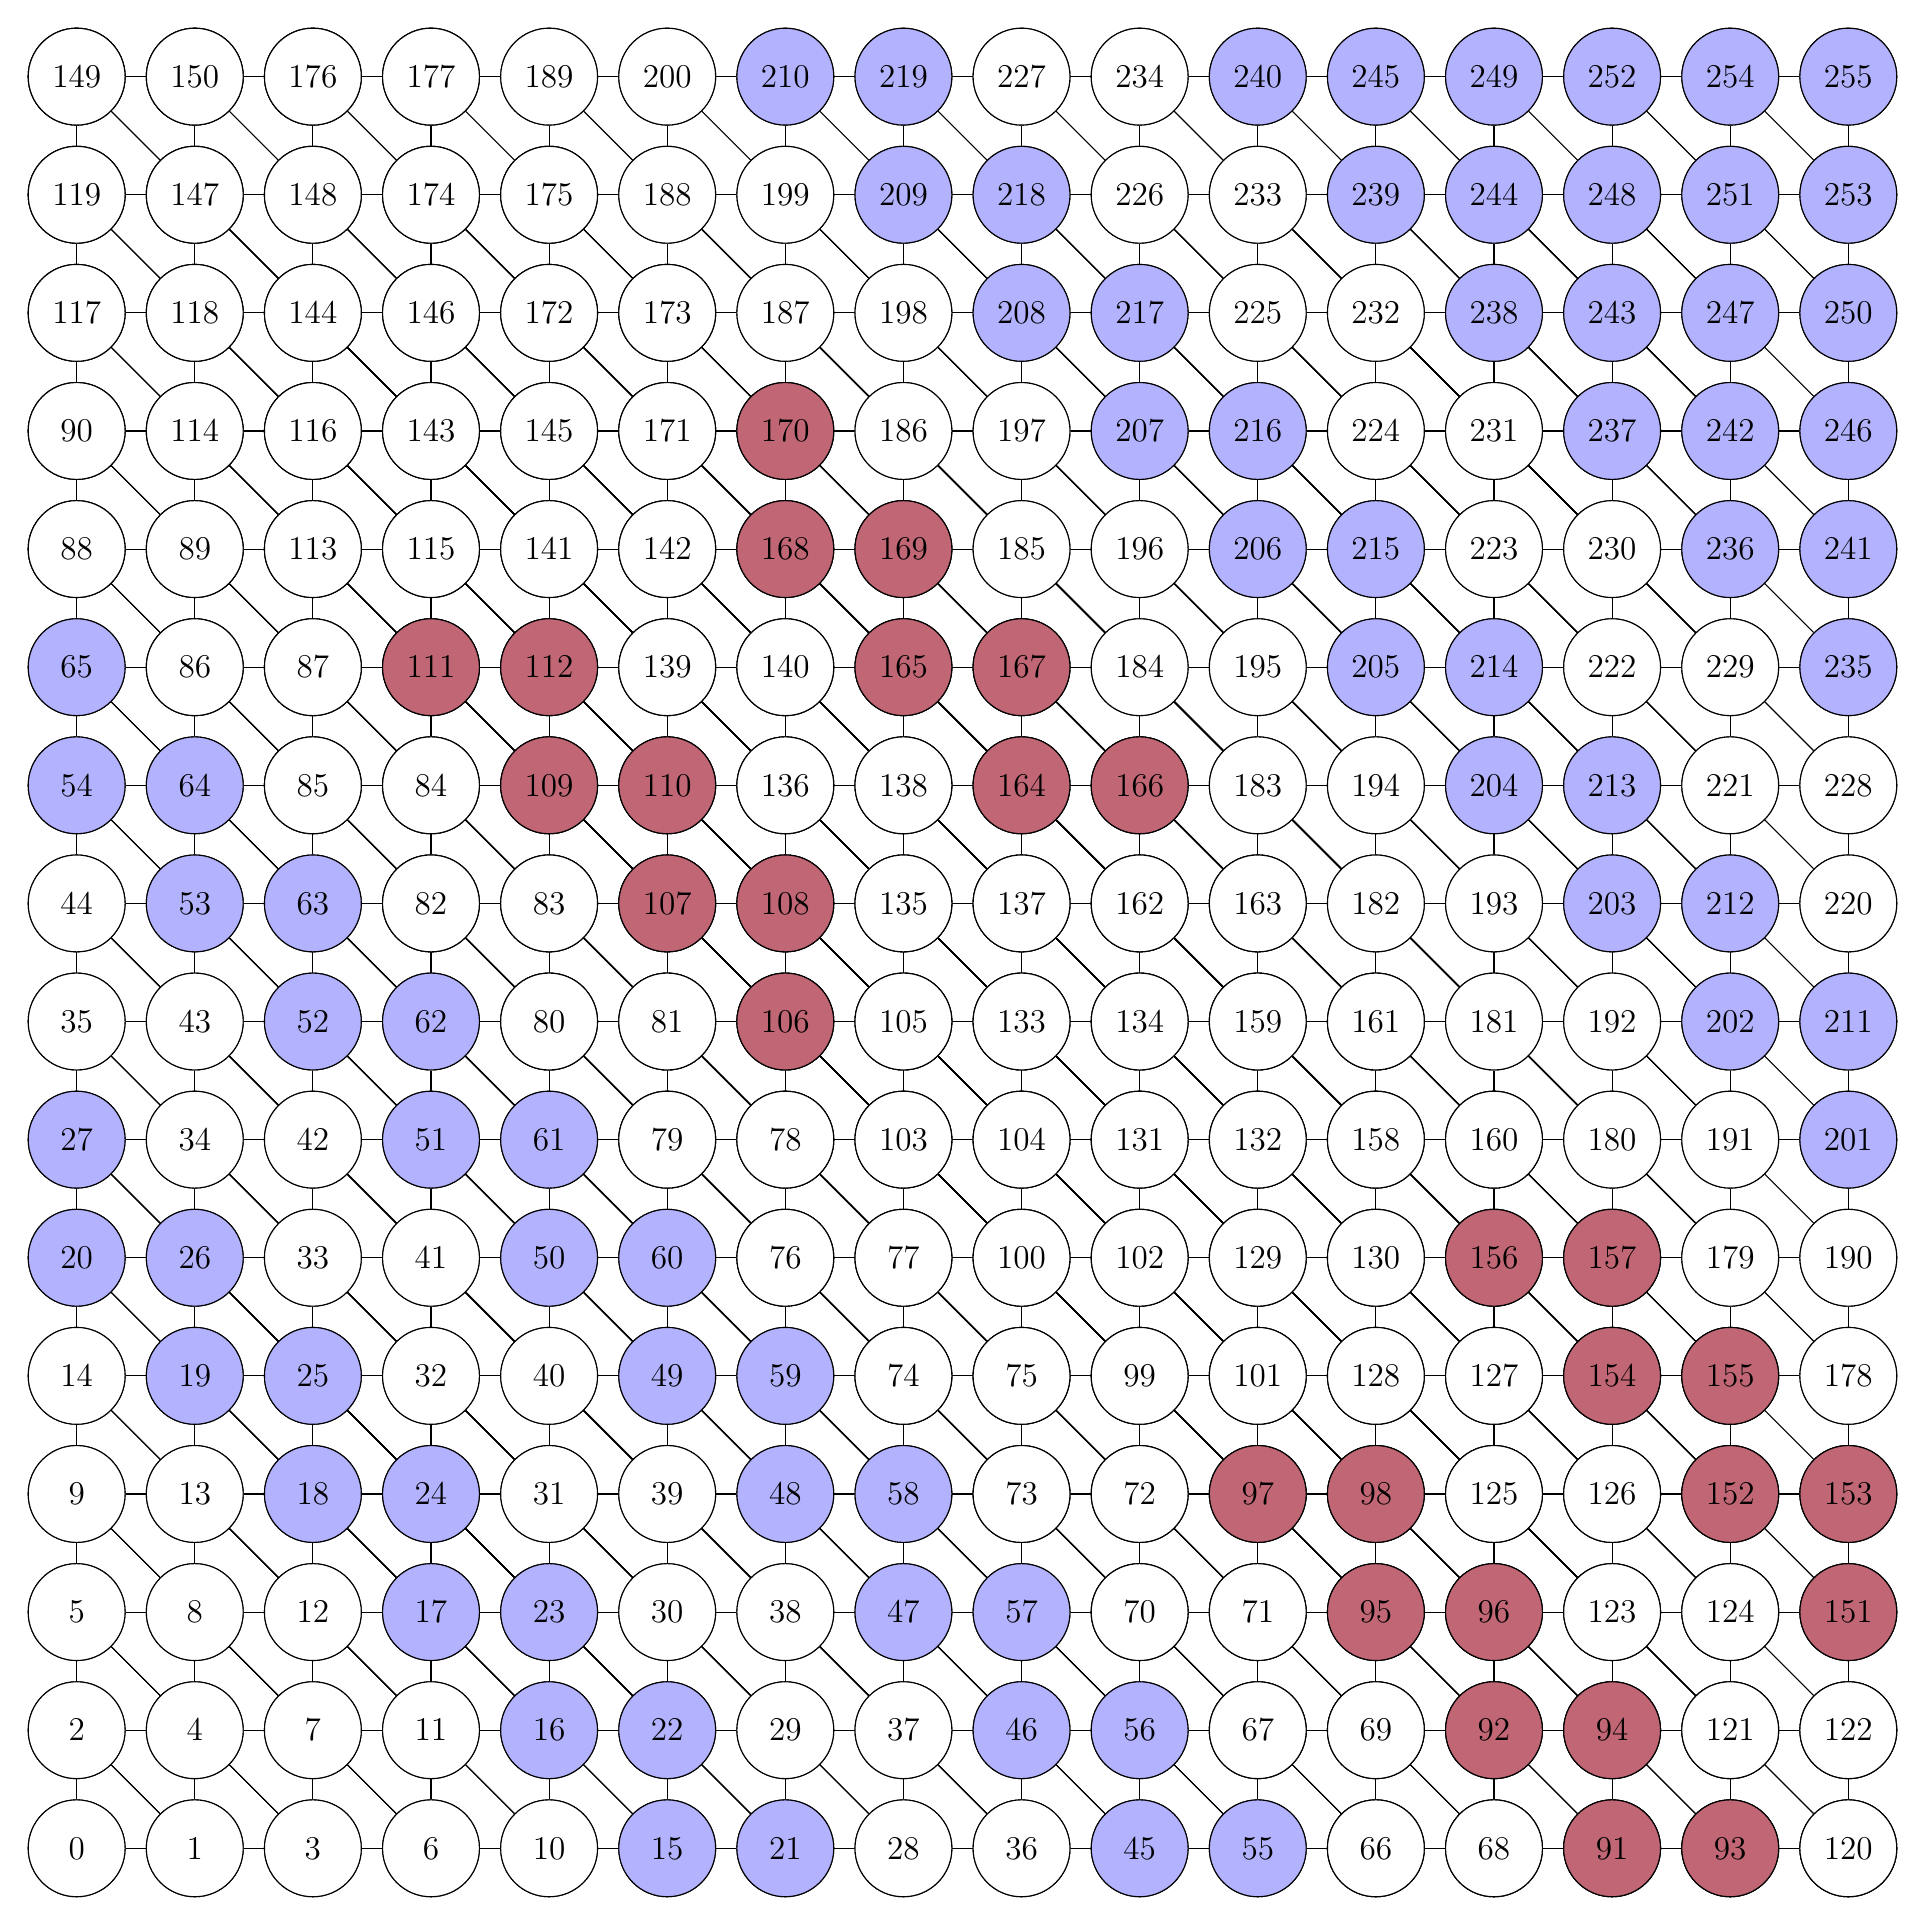
\begin{tikzpicture}[redstyle/.style={circle,draw,fill=white,minimum size=35}, bluestyle/.style={circle,draw,fill=blue!30!white,minimum size=35}, amberstyle/.style={circle,draw,fill=white,minimum size=35}, magentastyle/.style={circle,draw,fill=white,minimum size=35}, carminestyle/.style={circle,draw,fill=carmine!60!white,minimum size=35}, cyanstyle/.style={circle,draw,fill=white,minimum size=35}]
	\foreach \x in {0,...,\size}
	\foreach \y in {0,...,\size} 
	{
		\pgfmathtruncatemacro{\sizepone}{\size+1 }
		\pgfmathtruncatemacro{\label}{\y*\sizepone + \x  }
		\pgfmathtruncatemacro{\labell}{(\y + \x)*(\y+\x+1)*0.5+\y  }
		\pgfmathtruncatemacro{\labelu}{((\size+1)*(\size+1)-1) - (((\size*2) - \y - \x)*((\size*2) - \y-\x + 1)*0.5+ \size-\y)  }
		\pgfmathtruncatemacro{\level}{\y + \x  }
		\pgfmathtruncatemacro{\yinv}{\size - \y }
	
	
		\pgfmathparse{\color[\level]}
		\edef\currCOLOR{\pgfmathresult}
		\node[\currCOLOR]  (\label) at (1.5*\x,1.5*\y) { \ifthenelse{\x > \yinv} {\large{\labelu}} {\large{\labell}}} ;
		;}
	
	\foreach \x in {0,...,\size}
	{
		\pgfmathtruncatemacro{\sizemone}{\size-1 }
		\pgfmathtruncatemacro{\sizepone}{\size+1 }
		\foreach \y [count=\yi] in {0,...,\sizemone}  
		{
			\pgfmathtruncatemacro{\labelone}{\y*\sizepone + \x  }
			\pgfmathtruncatemacro{\labeltwo}{\yi*\sizepone + \x  }
			\pgfmathtruncatemacro{\labelthree}{\x*\sizepone + \y  }
			\pgfmathtruncatemacro{\labelfour}{\x*\sizepone + \yi  }
			\draw (\labelone)--(\labeltwo) (\labelthree)--(\labelfour) ;
			\draw (\labelone)-- (\labelthree);
		}
	}
	
	\foreach \x in {0,...,\size}
	\foreach \y in {0,...,\size} 
	{
		\pgfmathtruncatemacro{\sizepone}{\size+1 }
		\pgfmathtruncatemacro{\label}{\y*\sizepone + \x  }
		\pgfmathtruncatemacro{\labell}{(\y + \x)*(\y+\x+1)*0.5+\y  }
		\pgfmathtruncatemacro{\labelu}{((\size+1)*(\size+1)-1) - (((\size*2) - \y - \x)*((\size*2) - \y-\x + 1)*0.5+ \size-\y)  }
		\pgfmathtruncatemacro{\level}{\y + \x  }
		\pgfmathtruncatemacro{\yinv}{\size - \y }
		
		\pgfmathparse{\color[\level]}
		\edef\currCOLOR{\pgfmathresult}
		\node[\currCOLOR]  (\label) at (1.5*\x,1.5*\y) { \ifthenelse{\x > \yinv} {\large{\labelu}} {\large{\labell}}} ;
		;}
	
		\newcounter{nodenumber}
		\foreach \zx in {0,1}
		{\pgfmathtruncatemacro{\tmp}{2+\zx }
		\foreach \y in {0,...,\tmp} 
		{
			\pgfmathtruncatemacro{\x}{11+\zx-\y }
			\pgfmathtruncatemacro{\sizepone}{\size+1 }
			\pgfmathtruncatemacro{\label}{\y*\sizepone + \x  }
			\pgfmathtruncatemacro{\labell}{(\y + \x)*(\y+\x+1)*0.5+\y  }
			\pgfmathtruncatemacro{\labelu}{((\size+1)*(\size+1)-1) - (((\size*2) - \y - \x)*((\size*2) - \y-\x + 1)*0.5+ \size-\y)  }
			\pgfmathtruncatemacro{\level}{\y + \x  }
			\pgfmathtruncatemacro{\yinv}{\size - \y }

			\pgfmathparse{\labelStwo[\arabic{nodenumber}]}
			\edef\label{\pgfmathresult}
			\stepcounter{nodenumber}
			\node[amberstyle] at (1.5*\x,1.5*\y) { \large{\label} };% \ifthenelse{\x > \yinv} {\large{\labelu}} {\large{\labell}}} ;
		;}
		}

		\foreach \zx in {0,1}
		{\pgfmathtruncatemacro{\tmpS}{3+\zx }
		\pgfmathtruncatemacro{\tmpE}{5+\zx }
			\foreach \y in {\tmpS,...,\tmpE} 
			{
				\pgfmathtruncatemacro{\x}{11+\zx-\y }
				\pgfmathtruncatemacro{\sizepone}{\size+1 }
				\pgfmathtruncatemacro{\label}{\y*\sizepone + \x  }
				\pgfmathtruncatemacro{\labell}{(\y + \x)*(\y+\x+1)*0.5+\y  }
				\pgfmathtruncatemacro{\labelu}{((\size+1)*(\size+1)-1) - (((\size*2) - \y - \x)*((\size*2) - \y-\x + 1)*0.5+ \size-\y)  }
				\pgfmathtruncatemacro{\level}{\y + \x  }
				\pgfmathtruncatemacro{\yinv}{\size - \y }
				
				\pgfmathparse{\labelStwo[\arabic{nodenumber}]}
				\edef\label{\pgfmathresult}
				\stepcounter{nodenumber}
				\node[magentastyle] at (1.5*\x,1.5*\y) { \large{\label} } ;
				;}
		}
		\foreach \zx in {0,1}
		{\pgfmathtruncatemacro{\tmpS}{6+\zx }
			\pgfmathtruncatemacro{\tmpE}{8+\zx }
			\foreach \y in {\tmpS,...,\tmpE} 
			{
				\pgfmathtruncatemacro{\x}{11+\zx-\y }
				\pgfmathtruncatemacro{\sizepone}{\size+1 }
				\pgfmathtruncatemacro{\label}{\y*\sizepone + \x  }
				\pgfmathtruncatemacro{\labell}{(\y + \x)*(\y+\x+1)*0.5+\y  }
				\pgfmathtruncatemacro{\labelu}{((\size+1)*(\size+1)-1) - (((\size*2) - \y - \x)*((\size*2) - \y-\x + 1)*0.5+ \size-\y)  }
				\pgfmathtruncatemacro{\level}{\y + \x  }
				\pgfmathtruncatemacro{\yinv}{\size - \y }
				
				\pgfmathparse{\labelStwo[\arabic{nodenumber}]}
				\edef\label{\pgfmathresult}
				\stepcounter{nodenumber}
				\node[amberstyle] at (1.5*\x,1.5*\y) { \large{\label} } ;
				;}
		}
		\foreach \zx in {0,1}
		{\pgfmathtruncatemacro{\tmpS}{9+\zx }
			\pgfmathtruncatemacro{\tmpE}{11+\zx }
			\foreach \y in {\tmpS,...,\tmpE} 
			{
				\pgfmathtruncatemacro{\x}{11+\zx-\y }
				\pgfmathtruncatemacro{\sizepone}{\size+1 }
				\pgfmathtruncatemacro{\label}{\y*\sizepone + \x  }
				\pgfmathtruncatemacro{\labell}{(\y + \x)*(\y+\x+1)*0.5+\y  }
				\pgfmathtruncatemacro{\labelu}{((\size+1)*(\size+1)-1) - (((\size*2) - \y - \x)*((\size*2) - \y-\x + 1)*0.5+ \size-\y)  }
				\pgfmathtruncatemacro{\level}{\y + \x  }
				\pgfmathtruncatemacro{\yinv}{\size - \y }
				
				\pgfmathparse{\labelStwo[\arabic{nodenumber}]}
				\edef\label{\pgfmathresult}
				\stepcounter{nodenumber}
				\node[magentastyle] at (1.5*\x,1.5*\y) { \large{\label} } ;
				;}
		}
		\foreach \zx in {0,1}
		{\pgfmathtruncatemacro{\tmpS}{0 }
			\pgfmathtruncatemacro{\tmpE}{3}
			\foreach \y in {\tmpS,...,\tmpE} 
			{
				\pgfmathtruncatemacro{\x}{13+\zx-\y }
				\pgfmathtruncatemacro{\sizepone}{\size+1 }
				\pgfmathtruncatemacro{\label}{\y*\sizepone + \x  }
				\pgfmathtruncatemacro{\labell}{(\y + \x)*(\y+\x+1)*0.5+\y  }
				\pgfmathtruncatemacro{\labelu}{((\size+1)*(\size+1)-1) - (((\size*2) - \y - \x)*((\size*2) - \y-\x + 1)*0.5+ \size-\y)  }
				\pgfmathtruncatemacro{\level}{\y + \x  }
				\pgfmathtruncatemacro{\yinv}{\size - \y }
				
				\pgfmathparse{\labelStwo[\arabic{nodenumber}]}
				\edef\label{\pgfmathresult}
				\stepcounter{nodenumber}				
				\node[carminestyle] at (1.5*\x,1.5*\y) { \large{\label}} ;
				;}
		}
		\foreach \zx in {0,1}
		{\pgfmathtruncatemacro{\tmpS}{4 }
			\pgfmathtruncatemacro{\tmpE}{6+\zx}
			\foreach \y in {\tmpS,...,\tmpE} 
			{
				\pgfmathtruncatemacro{\x}{13+\zx-\y }
				\pgfmathtruncatemacro{\sizepone}{\size+1 }
				\pgfmathtruncatemacro{\label}{\y*\sizepone + \x  }
				\pgfmathtruncatemacro{\labell}{(\y + \x)*(\y+\x+1)*0.5+\y  }
				\pgfmathtruncatemacro{\labelu}{((\size+1)*(\size+1)-1) - (((\size*2) - \y - \x)*((\size*2) - \y-\x + 1)*0.5+ \size-\y)  }
				\pgfmathtruncatemacro{\level}{\y + \x  }
				\pgfmathtruncatemacro{\yinv}{\size - \y }
				
				\pgfmathparse{\labelStwo[\arabic{nodenumber}]}
				\edef\label{\pgfmathresult}
				\stepcounter{nodenumber}	
				\node[cyanstyle] at (1.5*\x,1.5*\y) { \large{\label}} ;
				;}
		}
		\foreach \zx in {0,1}
		{\pgfmathtruncatemacro{\tmpS}{7+\zx }
			\pgfmathtruncatemacro{\tmpE}{10}
			\foreach \y in {\tmpS,...,\tmpE} 
			{
				\pgfmathtruncatemacro{\x}{13+\zx-\y }
				\pgfmathtruncatemacro{\sizepone}{\size+1 }
				\pgfmathtruncatemacro{\label}{\y*\sizepone + \x  }
				\pgfmathtruncatemacro{\labell}{(\y + \x)*(\y+\x+1)*0.5+\y  }
				\pgfmathtruncatemacro{\labelu}{((\size+1)*(\size+1)-1) - (((\size*2) - \y - \x)*((\size*2) - \y-\x + 1)*0.5+ \size-\y)  }
				\pgfmathtruncatemacro{\level}{\y + \x  }
				\pgfmathtruncatemacro{\yinv}{\size - \y }
				
				\pgfmathparse{\labelStwo[\arabic{nodenumber}]}
				\edef\label{\pgfmathresult}
				\stepcounter{nodenumber}	
				\node[carminestyle] at (1.5*\x,1.5*\y) { \large{\label}} ;
				;}
		}
		\foreach \zx in {0,1}
		{\pgfmathtruncatemacro{\tmpS}{11 }
			\pgfmathtruncatemacro{\tmpE}{13+\zx}
			\foreach \y in {\tmpS,...,\tmpE} 
			{
				\pgfmathtruncatemacro{\x}{13+\zx-\y }
				\pgfmathtruncatemacro{\sizepone}{\size+1 }
				\pgfmathtruncatemacro{\label}{\y*\sizepone + \x  }
				\pgfmathtruncatemacro{\labell}{(\y + \x)*(\y+\x+1)*0.5+\y  }
				\pgfmathtruncatemacro{\labelu}{((\size+1)*(\size+1)-1) - (((\size*2) - \y - \x)*((\size*2) - \y-\x + 1)*0.5+ \size-\y)  }
				\pgfmathtruncatemacro{\level}{\y + \x  }
				\pgfmathtruncatemacro{\yinv}{\size - \y }
				
				\pgfmathparse{\labelStwo[\arabic{nodenumber}]}
				\edef\label{\pgfmathresult}
				\stepcounter{nodenumber}	
				\node[cyanstyle] at (1.5*\x,1.5*\y) { \large{\label}} ;
				;}
		}
		
		\foreach \zx in {0,1}
		{\pgfmathtruncatemacro{\tmpS}{\zx }
			\pgfmathtruncatemacro{\tmpE}{3+\zx }
			\foreach \y in {\tmpS,...,\tmpE} 
			{
				\pgfmathtruncatemacro{\x}{15+\zx-\y }
				\pgfmathtruncatemacro{\sizepone}{\size+1 }
				\pgfmathtruncatemacro{\label}{\y*\sizepone + \x  }
				\pgfmathtruncatemacro{\labell}{(\y + \x)*(\y+\x+1)*0.5+\y  }
				\pgfmathtruncatemacro{\labelu}{((\size+1)*(\size+1)-1) - (((\size*2) - \y - \x)*((\size*2) - \y-\x + 1)*0.5+ \size-\y)  }
				\pgfmathtruncatemacro{\level}{\y + \x  }
				\pgfmathtruncatemacro{\yinv}{\size - \y }
				
				\pgfmathparse{\labelStwo[\arabic{nodenumber}]}
				\edef\label{\pgfmathresult}
				\stepcounter{nodenumber}
				\node[amberstyle] at (1.5*\x,1.5*\y) {\large{\label}} ;
				;}
		}
		\foreach \zx in {0,1}
		{\pgfmathtruncatemacro{\tmpS}{4+\zx }
			\pgfmathtruncatemacro{\tmpE}{7 }
			\foreach \y in {\tmpS,...,\tmpE} 
			{
				\pgfmathtruncatemacro{\x}{15+\zx-\y }
				\pgfmathtruncatemacro{\sizepone}{\size+1 }
				\pgfmathtruncatemacro{\label}{\y*\sizepone + \x  }
				\pgfmathtruncatemacro{\labell}{(\y + \x)*(\y+\x+1)*0.5+\y  }
				\pgfmathtruncatemacro{\labelu}{((\size+1)*(\size+1)-1) - (((\size*2) - \y - \x)*((\size*2) - \y-\x + 1)*0.5+ \size-\y)  }
				\pgfmathtruncatemacro{\level}{\y + \x  }
				\pgfmathtruncatemacro{\yinv}{\size - \y }
				
				\pgfmathparse{\labelStwo[\arabic{nodenumber}]}
				\edef\label{\pgfmathresult}
				\stepcounter{nodenumber}				
				\node[magentastyle] at (1.5*\x,1.5*\y) {\large{\label}} ;
				;}
		}
		\foreach \zx in {0,1}
		{\pgfmathtruncatemacro{\tmpS}{8 }
			\pgfmathtruncatemacro{\tmpE}{11}
			\foreach \y in {\tmpS,...,\tmpE} 
			{
				\pgfmathtruncatemacro{\x}{15+\zx-\y }
				\pgfmathtruncatemacro{\sizepone}{\size+1 }
				\pgfmathtruncatemacro{\label}{\y*\sizepone + \x  }
				\pgfmathtruncatemacro{\labell}{(\y + \x)*(\y+\x+1)*0.5+\y  }
				\pgfmathtruncatemacro{\labelu}{((\size+1)*(\size+1)-1) - (((\size*2) - \y - \x)*((\size*2) - \y-\x + 1)*0.5+ \size-\y)  }
				\pgfmathtruncatemacro{\level}{\y + \x  }
				\pgfmathtruncatemacro{\yinv}{\size - \y }
				
				\pgfmathparse{\labelStwo[\arabic{nodenumber}]}
				\edef\label{\pgfmathresult}
				\stepcounter{nodenumber}			
				\node[amberstyle] at (1.5*\x,1.5*\y) {\large{\label}} ;
				;}
		}
		\foreach \zx in {0,1}
		{\pgfmathtruncatemacro{\tmpS}{12 }
			\pgfmathtruncatemacro{\tmpE}{15}
			\foreach \y in {\tmpS,...,\tmpE} 
			{
				\pgfmathtruncatemacro{\x}{15+\zx-\y }
				\pgfmathtruncatemacro{\sizepone}{\size+1 }
				\pgfmathtruncatemacro{\label}{\y*\sizepone + \x  }
				\pgfmathtruncatemacro{\labell}{(\y + \x)*(\y+\x+1)*0.5+\y  }
				\pgfmathtruncatemacro{\labelu}{((\size+1)*(\size+1)-1) - (((\size*2) - \y - \x)*((\size*2) - \y-\x + 1)*0.5+ \size-\y)  }
				\pgfmathtruncatemacro{\level}{\y + \x  }
				\pgfmathtruncatemacro{\yinv}{\size - \y }
				
				\pgfmathparse{\labelStwo[\arabic{nodenumber}]}
				\edef\label{\pgfmathresult}
				\stepcounter{nodenumber}							
				\node[magentastyle] at (1.5*\x,1.5*\y) { \large{\label}} ;
				;}
		}
		\foreach \zx in {0,1}
		{\pgfmathtruncatemacro{\tmpS}{2+\zx }
			\pgfmathtruncatemacro{\tmpE}{5}
			\foreach \y in {\tmpS,...,\tmpE} 
			{
				\pgfmathtruncatemacro{\x}{17+\zx-\y }
				\pgfmathtruncatemacro{\sizepone}{\size+1 }
				\pgfmathtruncatemacro{\label}{\y*\sizepone + \x  }
				\pgfmathtruncatemacro{\labell}{(\y + \x)*(\y+\x+1)*0.5+\y  }
				\pgfmathtruncatemacro{\labelu}{((\size+1)*(\size+1)-1) - (((\size*2) - \y - \x)*((\size*2) - \y-\x + 1)*0.5+ \size-\y)  }
				\pgfmathtruncatemacro{\level}{\y + \x  }
				\pgfmathtruncatemacro{\yinv}{\size - \y }
				
				\pgfmathparse{\labelStwo[\arabic{nodenumber}]}
				\edef\label{\pgfmathresult}
				\stepcounter{nodenumber}					
				\node[carminestyle] at (1.5*\x,1.5*\y) { \large{\label}} ;
				;}
		}
		\foreach \zx in {0,1}
		{\pgfmathtruncatemacro{\tmpS}{6 }
			\pgfmathtruncatemacro{\tmpE}{8}
			\foreach \y in {\tmpS,...,\tmpE} 
			{
				\pgfmathtruncatemacro{\x}{17+\zx-\y }
				\pgfmathtruncatemacro{\sizepone}{\size+1 }
				\pgfmathtruncatemacro{\label}{\y*\sizepone + \x  }
				\pgfmathtruncatemacro{\labell}{(\y + \x)*(\y+\x+1)*0.5+\y  }
				\pgfmathtruncatemacro{\labelu}{((\size+1)*(\size+1)-1) - (((\size*2) - \y - \x)*((\size*2) - \y-\x + 1)*0.5+ \size-\y)  }
				\pgfmathtruncatemacro{\level}{\y + \x  }
				\pgfmathtruncatemacro{\yinv}{\size - \y }
				
				\pgfmathparse{\labelStwo[\arabic{nodenumber}]}
				\edef\label{\pgfmathresult}
				\stepcounter{nodenumber}						
				\node[cyanstyle] at (1.5*\x,1.5*\y) { \large{\label}} ;
				;}
		}
		\foreach \zx in {0,1}
		{\pgfmathtruncatemacro{\tmpS}{9 }
			\pgfmathtruncatemacro{\tmpE}{11+\zx}
			\foreach \y in {\tmpS,...,\tmpE} 
			{
				\pgfmathtruncatemacro{\x}{17+\zx-\y }
				\pgfmathtruncatemacro{\sizepone}{\size+1 }
				\pgfmathtruncatemacro{\label}{\y*\sizepone + \x  }
				\pgfmathtruncatemacro{\labell}{(\y + \x)*(\y+\x+1)*0.5+\y  }
				\pgfmathtruncatemacro{\labelu}{((\size+1)*(\size+1)-1) - (((\size*2) - \y - \x)*((\size*2) - \y-\x + 1)*0.5+ \size-\y)  }
				\pgfmathtruncatemacro{\level}{\y + \x  }
				\pgfmathtruncatemacro{\yinv}{\size - \y }
				
				\pgfmathparse{\labelStwo[\arabic{nodenumber}]}
				\edef\label{\pgfmathresult}
				\stepcounter{nodenumber}				
				\node[carminestyle] at (1.5*\x,1.5*\y) { \large{\label}} ;
				;}
		}
		\foreach \zx in {0,1}
		{\pgfmathtruncatemacro{\tmpS}{12+\zx }
			\pgfmathtruncatemacro{\tmpE}{15}
			\foreach \y in {\tmpS,...,\tmpE} 
			{
				\pgfmathtruncatemacro{\x}{17+\zx-\y }
				\pgfmathtruncatemacro{\sizepone}{\size+1 }
				\pgfmathtruncatemacro{\label}{\y*\sizepone + \x  }
				\pgfmathtruncatemacro{\labell}{(\y + \x)*(\y+\x+1)*0.5+\y  }
				\pgfmathtruncatemacro{\labelu}{((\size+1)*(\size+1)-1) - (((\size*2) - \y - \x)*((\size*2) - \y-\x + 1)*0.5+ \size-\y)  }
				\pgfmathtruncatemacro{\level}{\y + \x  }
				\pgfmathtruncatemacro{\yinv}{\size - \y }
				
				\pgfmathparse{\labelStwo[\arabic{nodenumber}]}
				\edef\label{\pgfmathresult}
				\stepcounter{nodenumber}				
				\node[cyanstyle] at (1.5*\x,1.5*\y) { \large{\label}} ;
				;}
		}
	%	\draw [white] (0.1,-0.5) rectangle (0.2,-1.5);
	\end{tikzpicture}

\end{document}  